\documentclass{article}
\usepackage{fullpage}
\usepackage[portuguese]{babel}
\usepackage[utf8]{inputenc}
\usepackage[protrusion=true,expansion=true]{microtype}
\usepackage{graphicx}
\graphicspath{ {imgs/} }

\author{Henrique Aires Silva \\RA: 169574 \\ Turma T}

\newcommand{\horrule}[1]{\rule{\linewidth}{#1}} 	% Horizontal rule

\title{
  \usefont{OT1}{bch}{b}{n}
  \normalfont \normalsize \textsc{FEEC - Faculdade de Engenharia Elétrica e de Computação} \\
  \normalfont \normalsize EA871 - Lab. de Programação Básica de Sistemas Digitais
  \horrule{0.5pt} \\[1.0cm]
  \LARGE \textbf{Relatório do Experimento 2\\Ferramentas de Desenvolvimento de Software} \\[1.0cm]
  \horrule{2pt} \\[0.1cm]
}

\author{
  \normalfont 								\normalsize
  Henrique Aires Silva\\ \normalfont \normalsize RA: 169574 - Turma T\\[-3pt]		\normalsize
  \today
}
\date{}

\begin{document}
\maketitle

\section{Introdução}
Uma das etapas mais importantes do desenvolvimento de softwares embarcados é a rotina de testes (debug) junto ao Hardware selecionado. Esta tarefa nem sempre é a mais trivial, dado que o microcontrolador em que se deseja executar o software quase sempre não é o mesmo no qual se desenvolve. Além disso, por ser um ambiente de muito baixo nível lógico no sentido de abstrações, é praticamente inviavel testar o software desejado analisando as transações entre registradores internos do microcontrolador e mudanças lógicas de seus pinos.

Para amenizar alguns deste problemas e tornar a tarefa de desenvolvimento de software embarcado mais simples e acessível, foram criados softwares chamados de \textbf{IDEs} (Integrated Development Environments - Ambientes de Desenvolvimento Unificado) que tem por premissa abstrair o acesso aos registradores e informações de baixo nível do microcontrolador de modo que uma pessoa com minimos conhecimentos técnicos na área consiga com pouco esforço testar e corrigir, se necessário, seu software, focando seu esforço no desenvolvimento do algoritmo.

O IDE utilizado no curso de EA869 é conhecido como \textbf{CodeWarrior}, desenvolvido e mantido pela NXP (antiga Freescale). Nele estão presentes ferramentas de gerenciamento de projetos de software, editor de código, compilador e debugger, tudo em um mesmo ambiente.

Esta ferramenta é capaz de interfacear com o hardware da placa \textbf{FRDM-KL25}, que possui como componente principal o microcontrolador \textbf{MKL25Z128}, além de diversos periféricos, como converso USB-Serial, sensor capacitivo de toque, diversos pinos de propósito geral (GPIO) e um LED RGB, que será o foco deste experimento.

\section{Objetivo}

Durante este experimento, procurou-se a familiarização do aluno com a ferramenta de desenvolvimento de software embarcado CodeWarrior.

Para alcançar tal objetivo, foi proposto que fosse criado um simples programa que controle um LED RGB e pisque na cor branca (todas as cores acesas) em um intervalo de tempo fixo.

Com o objetivo de  estimular boas práticas de programação e incentivar o reuso de código, foi proposto que fosse desenvolvido um código modular, ou seja, com arquivos separados por função objetivo, de tal modo que este possa ser utilizado em outros projetos da disciplina no futuro caso necessário.

\section{Metodologia}
\subsection{LED RGB}
O LED RGB é composto por 3 LEDs de cores distintas (Azul, Verde e Vermelho) no mesmo encapsulamento com um anodo comum como mostrado na Figura \ref{led_rgb}. Desta forma é possível acioná-los independentemente controlando o nível de tensão em seu catodo.
Por estarem no mesmo encapsulamento é possível gerar diversas combinações de cores acionando os LEDs em conjunto, dado que sua luz emitida será difundida e misturada.

\begin{figure}[ht!]
\centering

\includegraphics[width=70mm]{rgb_led.png}
\caption{Esquema elétrico de um LED RGB com anodo comum \label{led_rgb}}
\end{figure}

No escopo deste experimento, não será explorado o conceito de modulação de pulso, que pode ser utilizado para gerar diversos tons de cores com apenas as 3 cores primárias, apenas o acionamento lógico (ligado ou desligado) dos catodos. Assim, temos um total de 7 cores distintas possíveis.

Para gerar uma luz branca por exemplo, é possível acionar todos os 3 LEDs.

\begin{figure}[ht!]
\centering
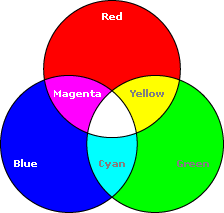
\includegraphics[width=40mm]{rgb_colors.png}
\caption{Diagrama mostrando as possíveis combinações de cores sólidas de um LED RGB \label{rgb_colors}}
\end{figure}

\subsubsection{Acionamento do LED RGB}

A conexão elétrica do LED RGB de anodo comum na placa MLK25Z128 segue um padrão bem conhecido, onde tem o pino comum ligado na alimentação positiva, e cada anodo sendo ligado em um pino independente do microcontrolador, com um resistor em série para limitar a corrente.

Este esquema é particularmente proveitoso pois ele contorna uma das dificuldades de todos os microcontroladores da atualidade, que é a capacidade baixa de fornecimento de corrente direto em pinos lógicos. Ou seja, se ligássemos o LED com o anodo ligado no pino lógico e o catodo no GND, dependendo do valor do resistor limitador, o controlador não conseguiria fornecer corrente suficiente para fazer o LED brilhar.

\begin{figure}[ht!]
\centering
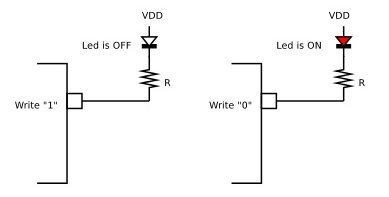
\includegraphics[width=85mm]{led_connect_sink.png}
\caption{Esquemático de uma ligação de um LED em um controlador usando lógica invertida \label{led_sink}}
\end{figure}


Por outro lado, os pinos lógicos tem uma grande capacidade de absorção de corrente, por conta de sua construção interna. Assim, podemos fazer a ligação mostrada na figura \ref{led_sink}

Desta forma, teremos uma lógica invertida no software, ou seja, para acionar o LED devemos escrever o nível lógico ''0'' no pino correspondente. Analogamente, para apagar o LED, basta escrever ''1'' em seu pino.

\subsection{Atrasos}

Como microcontroladores possuem períodos de relógio extremamente rápidos, da ordem de dezenas de nanosegundos, estes executam seus algoritmos de maneira quase imperceptível aos humanos.

Para que consigamos interpretar e interagir com o hardware, de forma a percebemos eventuais problemas, devemos fazer com o microcontrolador execute funções de atraso entre certos comandos que tem por objetivo a percepção humana, como o acionamento de um LED ou escrita de uma mensagem em um display.

Tais rotinas apenas fazem com que o processador fique parado num laço finito por um determinado tempo, sem realizar mais nenhum comando (não entram no escopo deste experimento as interrupções assíncronas), assim é possível que uma pessoa distingua o piscar de um LED por exemplo.


\section{Proposta de Solução}


\end{document}
